\documentclass{article}
\usepackage{graphicx}
\usepackage[english]{babel}
%\usepackage[a4paper]{geometry}
\usepackage[utf8]{inputenc}
\usepackage[T1]{fontenc}
\usepackage{needspace}
\usepackage{marginnote}
\renewcommand*{\marginfont}{\sffamily\footnotesize}
\usepackage{hyperref, graphicx, wrapfig}
\usepackage{imakeidx}
\usepackage{hyperref}
\makeindex[intoc]
\usepackage{pdfpages}
\usepackage{multirow}
\usepackage{color}
\usepackage{xcolor,colortbl}

\usepackage{tikz}
\usetikzlibrary{positioning}

\definecolor{Red}{rgb}{1,0,0}
\definecolor{Green}{rgb}{0,1,0}
\usepackage{tabularx}
\usepackage{caption}
\usepackage{background}

\backgroundsetup{
scale=1,
angle=34,
opacity=0.4,
contents={
\begin{tikzpicture}[remember picture,overlay]
 \path [left color = red!45,middle color = red!35, right color = white,rotate=1] (current page.south west)rectangle (current page.north east);   % Adjust the position of the logo.
\end{tikzpicture}\begin{tikzpicture}[remember picture,overlay]
 \path [left color = white,middle color = blue!20, right color = blue!40,rotate=13] (current page.south west)rectangle (current page.north east);   % Adjust the position of the logo.
\end{tikzpicture}\begin{tikzpicture}[remember picture,overlay]
 \path [left color = white,middle color = yellow!30, right color = white ,rotate=-13] (current page.south west)rectangle (current page.north east);   % Adjust the position of the logo.
\end{tikzpicture}}
}
%\newenvironment{overview}[3][]{
%  \needspace{10\baselineskip}
%  \begin{center}
%    { \renewcommand\textsuperscript[1]{}
%      \phantomsection\addcontentsline{toc}{section}
%      {\texorpdfstring{#2 (\emph{#3})}{#2 (#3)}}
%    }
%    {\large\bfseries #2\\}
%    \medskip
%    {#3\par}
%    \smallskip
%
%
%  {%
%  \bigskip
%  \hrule
%  \bigskip
%  }
%
%  \end{center}
%}
\newenvironment{overview}[4][]{
  \needspace{10\baselineskip}
  \begin{center}
    { \renewcommand\textsuperscript[1]{}
      \phantomsection\addcontentsline{toc}{section}
      {\texorpdfstring{#2 (\emph{#3})}{#2 (#3)}}
    }
    {\large\bfseries #2\\}
    \medskip
    {#3\par}
    \smallskip
    {\small #4\par}

  {%
  \bigskip
  \hrule
  \bigskip
  }
  \end{center}
}

\newcommand{\mc}[2]{\multicolumn{#1}{c}{#2}}
\newcommand{\mlcr}[4]{\multicolumn{#1}{#4}{\multirow{#2}{*}{#3}}}

\tikzstyle{blue} = [rectangle, draw, fill=blue!20,
 text width=0.4\textwidth, text centered, minimum height=4em]

\tikzstyle{red} = [rectangle, draw, fill=red!20,
 text width=0.4\textwidth, text centered, minimum height=4em]

\tikzstyle{timered} = [rectangle, draw, fill=red!20,
 text width=0.1\textwidth, text centered, minimum height=4em]

\tikzstyle{timeblue} = [rectangle, draw, fill=blue!20,
 text width=0.1\textwidth, text centered, minimum height=4em]

\tikzstyle{blue2} = [rectangle, draw, fill=blue!20,
 text width=0.4\textwidth, text centered, minimum height=6em]

\tikzstyle{red2} = [rectangle, draw, fill=red!20,
 text width=0.4\textwidth, text centered, minimum height=6em]

\tikzstyle{timered2} = [rectangle, draw, fill=red!20,
 text width=0.1\textwidth, text centered, minimum height=6em]

\tikzstyle{timeblue2} = [rectangle, draw, fill=blue!20,
 text width=0.1\textwidth, text centered, minimum height=6em]


\begin{document}

\newenvironment{changemargin}[2]{%
\begin{list}{}{%
\setlength{\topsep}{0pt}%
\setlength{\leftmargin}{#1}%
\setlength{\rightmargin}{#2}%
\setlength{\listparindent}{\parindent}%
\setlength{\itemindent}{\parindent}%
\setlength{\parsep}{\parskip}%
}%
\item[]}{\end{list}}

\begin{titlepage}
	\centering
	
\includegraphics[width=0.8\textwidth]{img/mat-mn-navn-eng.eps}\par\vspace{1cm}
	{\scshape\LARGE BIOMECHANICS OF LIVING SYSTEMS, FROM CELLS TO ORGANISMS \par}
	\vspace{1cm}
	{\scshape\Large Tøyen Hovedgård \\ Oslo Norway\par}
	\vspace{1.5cm}

\begin{changemargin}{-1cm}{-1cm}

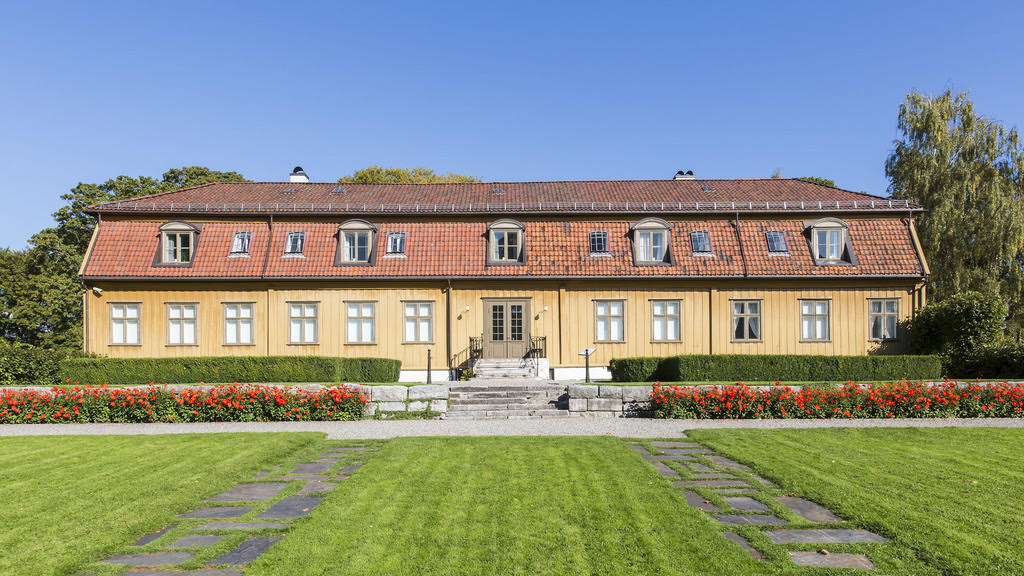
\includegraphics[scale=0.4]{img/hoved.jpg}

\centering
\vspace{0.5cm}
{\scshape\Large  Sponsors}
\vspace{0.5cm}




\includegraphics[scale=0.45]{01-UiO-Hovedlogo/English/UiO_Seal_B_ENG_cmyk.eps}\hspace*{2cm}

\includegraphics[scale=0.45]{img/logo.png}
\end{changemargin}

	\vfill

% Bottom of the page

\end{titlepage}


















\newcommand{\eventblock}[5]{
\node [#1,#2] (#3) {#4};
\node [time#1,left= of #3] (Time) {#5 }  ;  }
\begin{center}
\section*{PROGRAM}
\begin{changemargin}{-1cm}{-1cm}

\begin{tikzpicture}[node distance=-1pt, auto]
 % Place nodes

\eventblock{red}{}{Friday}{Program \\ Friday September 29 }{}
\eventblock{blue}{below= of Friday}{Registration}{Registration with coffee and danish}{09.00}
\eventblock{red}{below= of Registration}{Opening}{Opening \\ Dean Morten Dæhlen}{09.15}
\eventblock{blue}{below= of Opening}{SessionOne}{Susanne Liese \\
Aslak Tveito \\ Mattia Gazzola}{S1 \\ 09.30}
\eventblock{red}{below= of SessionOne}{BreakOne}{Break with coffee and softdrinks}{10.45}
\eventblock{blue}{below= of BreakOne}{SessionTwo}{Margarita Staykova \\ Gladys Massiera }{S2 \\ 11.10}
\eventblock{red}{below= of SessionTwo}{Lunch}{Lunch}{12.00}
\eventblock{blue2}{below= of Lunch}{SessionThree}{Liesbeth Janssen \\ Irep G\"ozen \\ Yasmine Meroz \\ Cinzia Progida}{S3 \\ 13.15}
\eventblock{red}{below= of SessionThree}{BreakTwo}{Break with coffee and fruits}{14.55}
\eventblock{blue}{below= of BreakTwo}{SessionFour}{Raymond E. Goldstein \\ Stig Ove Bøe \\ Guillaume Salbreux}{S4 \\ 15.15}
\eventblock{red}{below= of SessionFour}{Social}{Social gathering with snacks, beer and wine.}{16.30}
\eventblock{blue}{below= of Social}{Dinner}{Workshop dinner at \\ Trattoria Popolare}{19.00}


\eventblock{red}{right=2cm of Friday}{Saturday}{Program \\ Saturday September 30 }{}
\eventblock{blue2}{below= of Saturday}{SessionFive}{Marie Rognes \\ Alexandra Diem \\ M\'ar M\'asson \\ Federico Fenaroli}{S5 \\ 09.00}
\eventblock{red}{below= of SessionFive}{BreakThree}{Break with coffee, croissants and softdrinks}{  10.40}
\eventblock{blue}{below= of BreakThree}{SessionSix}{Klas Pettersen \\ Sylvie Lorthois \\ Paul Dommersnes}{S6 \\ 11.10}
\eventblock{red}{below= of SessionSix}{LunchTwo}{Lunch}{12.00}
\eventblock{blue2}{below= of LunchTwo}{Tour}{Guided Tour Munch Museum \\ 2 groups }{13.15}


\end{tikzpicture}
\end{changemargin}
\end{center}

\clearpage

\
\subsection*{\underline{The airport}}

\textbf{When you arrive at the airport} you need to
get to Oslo city center (Oslo S).
The fastest and easiest means of transportation to and from the airport
is by train. There are two different train operators, NSB
(Norwegian State Railway) and Flytoget (Airport Express Train).
There are some differences in price and
 and frequency of departures.
\textbf{Tickets for both NSB and Flytoget} can be bought at the airport
and at Oslo S in automatic ticket machines which accepts both cash
and credit cards.

\textbf{Traveling with NSB} is the cheapest
option whit a single ticket price
of 93 NOK. The frequency of departures varies but
usually there are at least 2 per hour and the time of travel is 23
 minutes. The times for departure is easy to find
both at the airport and at Oslo S.
At NSB it is also possible to buy your ticket
onboard the train at an additional cost of $40$NOK.
Pay attention to which stop to exit at (Oslo S/Gardermoen airport)
as this might not be the end stop for the train.

\textbf{Traveling with Flytoget} costs 180 NOK for a single ticket
but the frequency of departure per hour is 6, one every
ten minutes with a travel time of approximately 20 minutes.
Flytoget does not accept on-board payment!


\subsection*{\underline{Getting around in Oslo}}

The public transportation in Oslo is good with frequent
departures if you want
to take a bus, tram or subway. Buying tickets must be
done in advance and there are many places you can buy a
ticket. Oslo S, Narvesen, 7-eleven and Deli de Luca are some of the places.
A short "how-to" guide for getting to and from your hotel
 to the workshop related
locations (Fig.\ref{fig:Oslo}) follows below. Keep in mind that
the distances
between the different locations are not very large so if the
weather is nice, walking is recommended. If needed, taxi's
are a common sight in Oslo but if none are found you can order one
at tlf: +47 02323. Note that taxies are expensive in Norway.

\clearpage

\subsection*{\underline{Comfort Hotel Karl Johan}}

\begin{wrapfigure}{r}{0.4\textwidth}
\centering
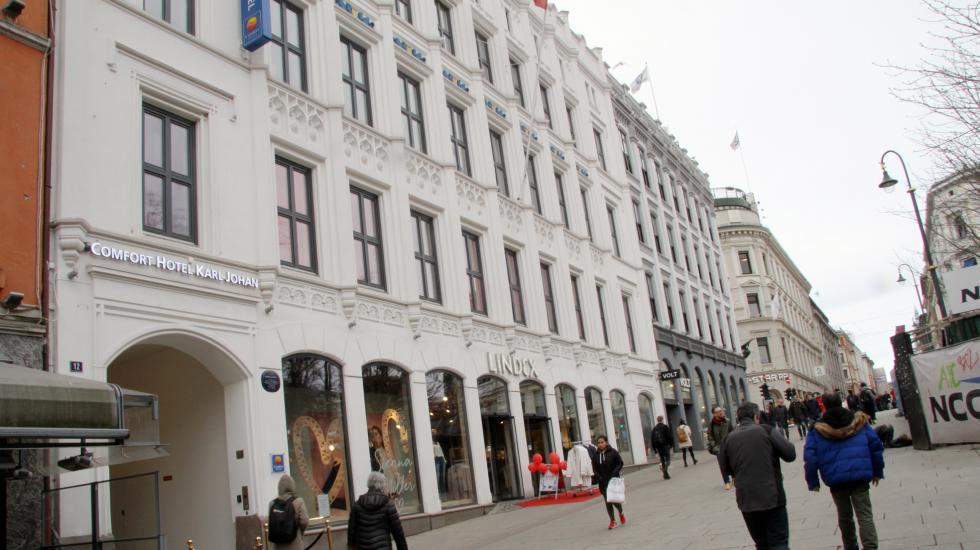
\includegraphics[scale=0.2]{img/comfort_karl_johan.jpg}
\caption{\label{fig:frog1}Exterior of Comfort Hotel Karl Johan.}
\end{wrapfigure}
The hotel is located at Karl Johans gate 12 near
the train station at Jernbanetorget.
This is also
a hub for public transportation in Oslo. \textbf{To get to
Tøyen hovedgård} where the workshop is taking place,
the best option is to take the subway from Jernbanetorget
to Tøyen and walk the remaining bit. The subway station
at Jernbanetorget is located under the shopping centre
Byporten and the entrances are clearly marked.
All subway trains,
\noindent 1-5, go to Tøyen from
Jernbanetorget in the eastward direction. \textbf{To get from
the restaurant, Trattoria Popolare,} you can take the tram. Lines
11, 12 and 13 will take you from Schous Plass to Jernbanetorget.



\subsection*{\underline{Scandic Vulkan}}
\begin{wrapfigure}{r}{0.42\textwidth}
\centering
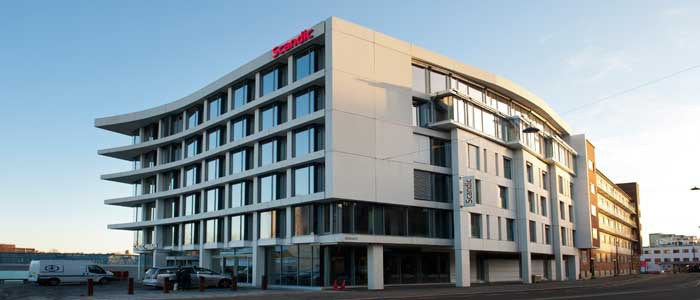
\includegraphics[width=0.45\textwidth, height=0.3\textwidth]{img/scandic-vulkan.jpg}
\caption{\label{fig:frog1}Exterior of Scandic Vulkan.}
\end{wrapfigure}
The hotel is located in Maridalsveien 13.
\textbf{The best way to get to Scandic Vulkan} from
Jernbanetorget is by bus. Lines 34 and 54 will take you
to the bus stop Telthusbakken which is located 100 meters
north of the hotel. \textbf{To get to Tøyen hovedgård}
you can take the bus back to Oslo S and from there take
the subway in the eastward direction to Tøyen. All subway
lines, 1-5, takes you there. \textbf{The restaurant, Trattoria Popolare,}
is only a 10 minute walk along the river
 from your hotel and this is also
the fastest way to get there.



\clearpage
\begin{center}


%WHAT TO DO
\section*{What to do in Oslo ?}
In Oslo there are many different tourist attractions, and we will present a few  popular sites. Attractions in Oslo can be found on \href{www.visitoslo.com}{www.visitoslo.com}.


\end{center}
\begin{wrapfigure}[9]{R}{0.5\textwidth}
    \centering
    \captionsetup{width=0.4\textwidth}
    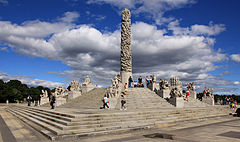
\includegraphics[width=0.5\textwidth]{img/Vigelansparken.jpg}%
     \caption{The monolith sculpute in the Park.}
\end{wrapfigure}

\section*{Vigeland Sculpture Park}

Vigeland Park is the world's largest sculpture park made by a single artist, and is one of Norway's most popular tourist attractions. The unique sculpture park is Gustav Vigeland's lifework with more than 200 sculptures in bronze, granite and wrought iron. The park is located a short 10 minute walk from the subway station Majorstuen.

\begin{wrapfigure}[10]{R}{0.5\textwidth}
    \centering
    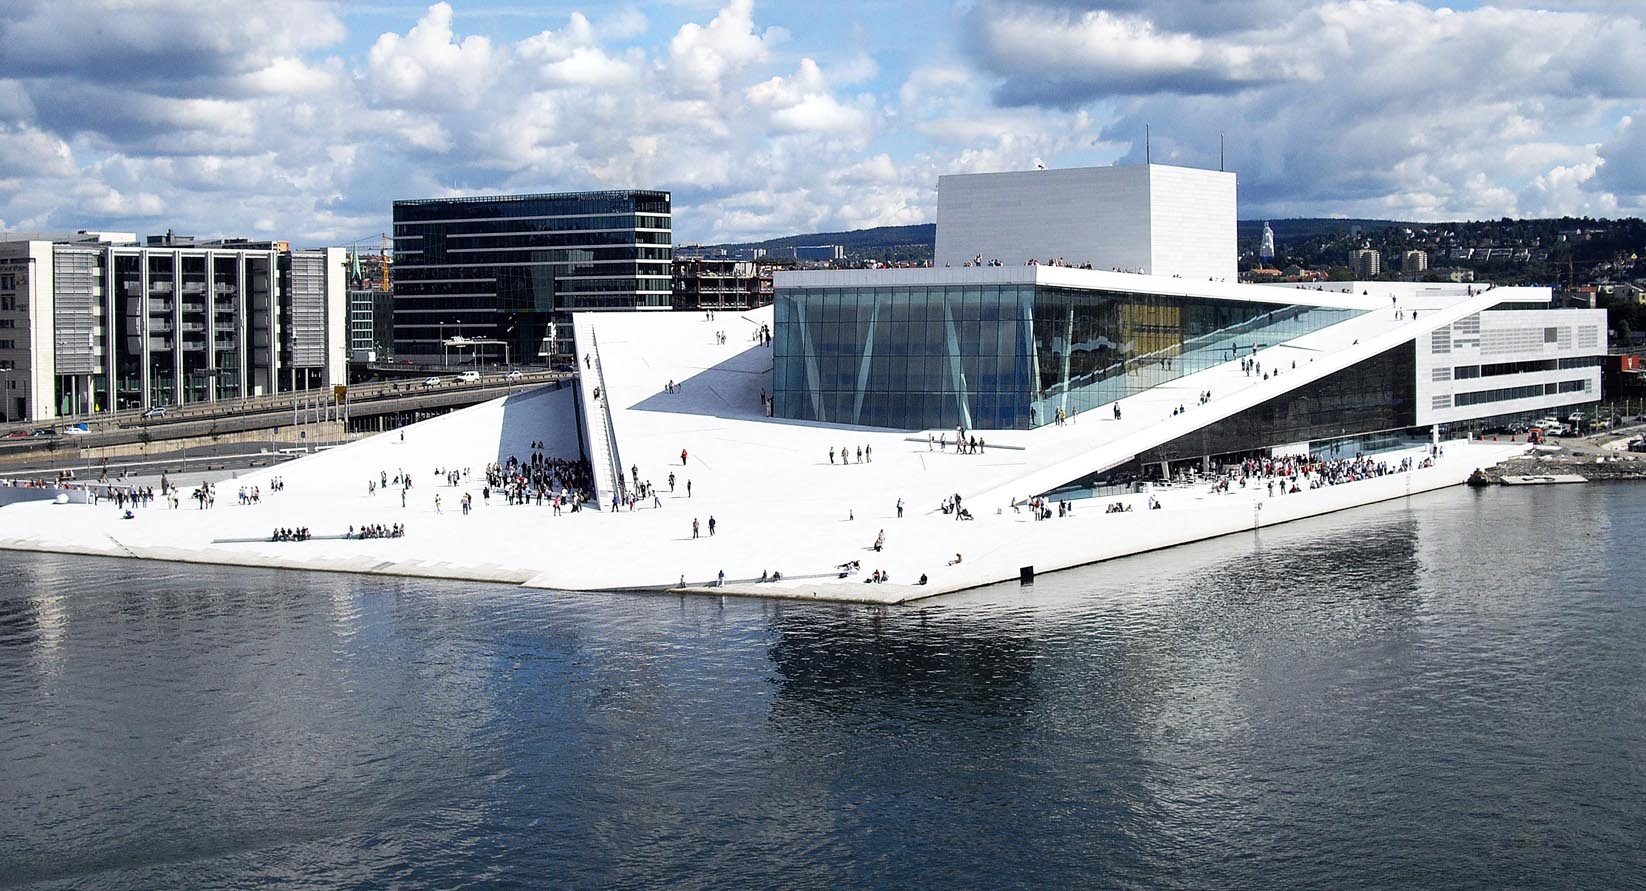
\includegraphics[width=0.5\textwidth]{img/operahouse.jpg}%
     \caption{Oslo Opera House }
\end{wrapfigure}

\vspace{1cm}

\section*{Opera House}
Oslo's Opera House is located right at the harbour, with an angled, white exterior that appears to rise from the water. It invites its visitors to climb its roof and enjoy panoramic views of Oslo and the fjord, all year round. \\
Large-scale windows at street level provide the public with glimpses of rehearsals and workshop activities. The building's interior is mainly oak, and the main hall is shaped like a horseshoe, reminiscent of classical theatres of the past. The opera is designed by the Norwegian architecture firm Snøhetta, and has received several prestigious awards. You can walk to the Opera House from the Jernbanetorget (central station) in about 15 minutes.

\clearpage

\section*{Gr\"unerløkka}
Through Oslo, from north to south, runs the river Akerselva. Along the river there are parklands and walking trails, but also remains of Oslo’s industrial history.
Gr\"unerløkka lies on the east side of the river, behind the old industrial buildings. The former factory district turned fashion hub, with laid-back cafes and galleries galore, Gr\"unerløkka is a colourful mix of old and new decor. Independent boutiques and design shops showcase Oslo’s more alternative side, with 19th-century buildings serving as a picturesque backdrop.

\bigskip
\bigskip

\begin{figure}[h]
    \centering
    \href{https://www.google.com/maps/d/edit?hl=no&hl=no&mid=1q9FpcHekR77D16V4eefgqkybvNc&ll=59.91839077669053%2C10.758429782339476&z=15}{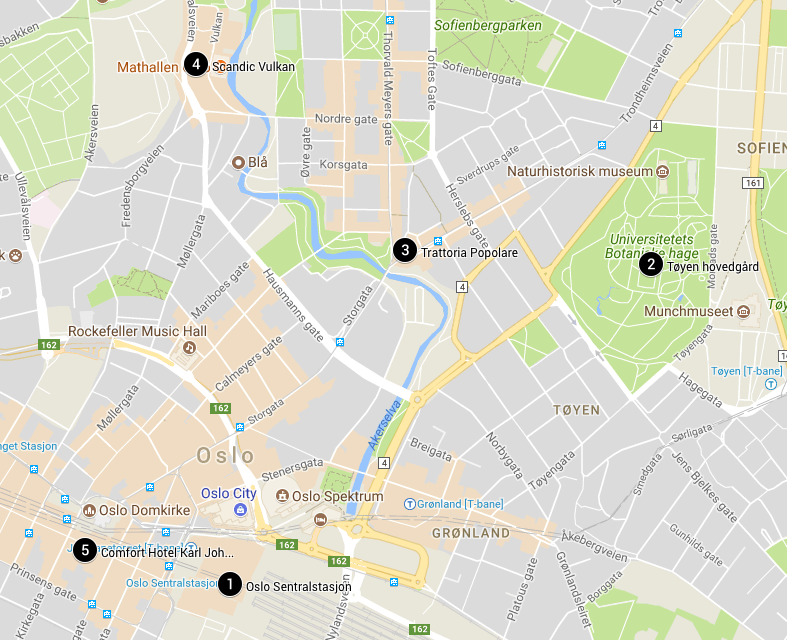
\includegraphics[width=1\linewidth, height=1\linewidth]{img/Oslo.png}}
    \caption{Locations of the 5 workshop related locations in Oslo.}
    \label{fig:Oslo}
\end{figure}




\clearpage



% ABSTRACTS

\includegraphics[scale=0.3]{img/mat-mn-navn-eng.eps}


\section*{Session 1}
\overview{Hydration Effects Turn a Highly Stretched Polymer from an Entropic into an Energetic Spring}{Susanne Liese}{Department of Mathematics, University of Oslo}{
Polyethylene glycol (PEG) is a structurally simple and nontoxic water-soluble polymer
that is widely used in medical and pharmaceutical applications as molecular linker
and spacer. In such applications, PEG’ s elastic response against conformational
deformations is key to its function. According to text-book knowledge, a polymer
reacts to the stretching of its end-to-end separation by a decrease in entropy that is
due to the reduction of available conformations, which is why polymers are commonly
called entropic springs. By a combination of single-molecule force spectroscopy
experiments with molecular dynamics simulations in explicit water, we show that
entropic hydration effects almost exactly compensate the chain conformational
entropy loss at high stretching. Our simulations reveal that this entropic
compensation is due to the stretching-induced release of water molecules that in the
relaxed state form double hydrogen bonds with PEG. As a consequence, the
stretching response of PEG is predominantly of energetic, not of entropic, origin at
high forces and caused by hydration effects, while PEG backbone deformations only
play a minor role. These findings demonstrate the importance of hydration for the
mechanics of macromolecules and constitute a case example that sheds light on the
antagonistic interplay of conformational and hydration degrees of freedom.}


\overview{A cell-based framework for numerical modeling of electrical conduction in cardiac tissue}{Aslak Tveito}{Simula Research Laboratory}{In every heartbeat, an electrical wave traverses the entire heart muscle, and in every heart cell,
this wave sets off an action potential that increases the transmembrane potential of the cell.
This leads to the release of large amounts of calcium from internal storage structures of the cell.
Increased cytosolic calcium concentration, in turn, leads to contraction of the cells, and the well
synchronized contraction of about nine billion cells underlie the pumping function of the heart.
The electrical wave originating in the Sino-atrial node and spreading, at high speed, throughout
the heart muscle is of vital importance of every human and perturbations to the wave – referred to as arrhythmias – can be life-threatening. Significant efforts are therefore invested in
understanding this wave and how dangerous perturbations can be avoided.
Over the last 60 years mathematical models have been used intensively to study electrical
conduction in the heart. The models involved are based on homogenization of the cardiac tissue
and are of reaction diffusion type where a parabolic equation is coupled to a large system of
ordinary differential equations defined in every point of the tissue. These models have been
very successful in providing a basic understanding of the properties of the excitation waves, and
have represented the level of accuracy that has been computationally feasible.
With increasing computing capacities, it has become clear that ever more realistic models can
be solved. Such models can increase insight into the astonishingly complex processes underlying
every heartbeat. In the present talk, we will discuss a cell-based framework for modeling the
electrical conduction system which avoids parts of the homogenization used in the classical
models. We will discuss the computational problems arising in the cell-based models and
provide some examples of simulations revealing new insight into electrical conduction through a
small number of cells.}


\overview{Computational design of artificial creatures}{Mattia Gazzola}{Department of Mechanical Science and Engineering, University of Illinois Urbana-Champaign}{We introduce an inverse design approach based on minimal theoretical modeling, direct numerical simulations and artificial intelligence for the investigation of animal locomotion. We will mostly focus on aquatic and terrestrial limbless creatures and discuss the identification of optimal swimming gaits and morphologies, as well as the design of cyborg creatures.}

\newpage
\section*{Session 2}


\overview{
Mechanics of the cell interface studied by supported lipid bilayers
}{Margarita Staykova}{Department of Physics, Durham University}{ The cell membrane undergoes complex morphological and surface area transformations while being confined to an underlying actin cortex, the membranes of neighboring cells or other extracellular structures. To understand the role of confinement in the membrane processes we adhere synthetic lipid bilayers to artificial substrates and subject them to perturbations that are common to the cell membrane - 1) substrate area changes, or 2) intake of extra lipids. Our results show that confined lipid bilayers regulate the arising changes in their lipid density either by the expulsion and absorption of lipid protrusions, such as tubes and vesicles, or by sliding over the substrate. Similar processes have been recently confirmed in living cells. We provide a theoretical framework that rationalizes the membrane behavior in terms of the membrane elasticity, and the adhesion and hydrodynamic interactions between the membrane and the substrate.
}


\overview{Biophysical approach of the mucociliary function: Mucus rheology and beating coordination}{Gladys Massiera}{Laboratoire Charles Coulomb (L2C), University of Montpellier}{The mucociliary function of the bronchial epithelium ensures the continuous clearance of the respiratory system, which relies on two main elements: mucus and cilia beating coordination.
We perform here a rheological characterization of mucus samples extracted from ALI (Air-liquid interface) cultures of bronchial epithelium. Our approach combines  macro- and micro-rheology techniques with the aim of quantifying the mucus viscoelastic properties at different length scales (from the size of bronchial cilia up to the scale on which mucus is transported)
}

\newpage
\section*{Session 3}
%Theory of Polymers and Soft Matter,
\overview{Membrane formation and compartmentalization in synthetic active matter}{Liesbeth M. C. Janssen}{Department of Applied Physics, Eindhoven University of Technology}{Active matter refers to systems whose constituent agents can move autonomously through the
consumption of energy. Such materials exhibit rich non-equilibrium dynamics and provide a framework
to understand the complex collective behavior seen in many living systems. In this talk, I will highlight
recent results of particle-resolved simulations of active rods that mimic cell-like properties such as
membrane formation and compartmentalization of particles. The crucial ingredients in our model are
the particles’ intrinsic self-propulsion, interparticle aligning interactions, and an inhomogeneous
motility field. We thus show that a minimal artificial active-matter system can self-organize into
structures reminiscent of biological patterns. Our predictions may be verified experimentally in e.g.
vibrated granular matter and other dry active systems with a spatially dependent self-propulsion speed.\\
\small{
Reference: J. Grauer, H. Löwen, and L.M.C. Janssen, Spontaneous membrane formation and self-
encapsulation of active rods in an inhomogeneous motility field, arXiv:1707.03405.}
}
\overview{Surface-Adhered Membranes: A physicochemical toolbox to investigate biochemical phenomena}{Irep G\"ozen}{Center for Molecular Medicine Norway, University of Oslo}{I will describe the generation, characterization and uses of a peculiar type of solid-supported model membrane: the self-spreading double bilayer. This type of solid-supported model membranes combines features and properties of a 2D lipid bilayer membrane, and a 3D phospholiposome. The double bilayer membrane, i.e. a fully closed, parallel stack of two lipid bilayers, is essentially a surface-adhered flat giant unilamellar vesicle with very small internal volume. I will explain how this structure can be manipulated to probe and migrate upon chemical or physical cues, and display dynamic feartues reminiscent of complex cell behavior. A number of examples will be shown, including formation of filopodia-like protrusions and ER-like lipidic networks as a response to chemical gradients; directed and reversible movement in a temperature gradient, which links biomembrane materials properties to fundamental properties of thin solid materials. One of the modes displays crackling noise dynamics, featuring suden intermittent bursts over a broad size range (avalanches), similar to earthquakes. I will finalize my talk showing how lipid membranes can be written on and deleted form solid substrates by using a microfluidic 'biopen'. I consider flat unilamellar vesicles as an experimental model system for studying various aspects of cell behavior as well as a nanotechnological platform, useful to construct mesoscale membrane architectures and networks.  }


\overview{Uncovering Organismal Memory Phenomena: From Cellular Chemotaxis to Plant Tropisms}{Yasmin Meroz}{School of Plant Sciences and Food Security, Tel Aviv University}{Statistical physics relates macroscopic dynamics of a system to the underlying microscopic physics through a probabilistic examination. In this talk I adopt this approach in the investigation of organismal memory phenomena. I study responses of biological organisms to external stimuli, with the aim of uncovering dominant physical mechanisms at the microscopic level, such as stochastic transport, first-passage processes, and mechanical couplings, to name a few. In particular, I focus on the example of cellular chemotaxis - the orientation of a biological cell in the direction of a chemical gradient. I show that a probabilistic minimal model of whole cell response dynamics to chemical cues, gives a mechanistic understanding of the complex phenomenon of directional memory. Predictions of our model are verified both numerically and experimentally, confirming that this approach is effective in providing crucial insight into the physics of complex biological systems.
}

\overview{2D or not 2D: Dimensional and mechanical cues in cell migration.}{Cinzia Anita Maria Progida}{
Department of Biosciences,
University of Oslo}{The movement of cells within the body, or cell migration, is fundamental for both physiological and
pathological processes including wound healing, immune response and cancer metastasis. Cell
motility involves the reorganization of the cytoskeleton and the movement of organelles, usually
triggered by external cues. Indeed, cells respond to biochemical or mechanical stimuli by activating
signaling pathways, re-organizing the cytoskeleton and generating forces. We study how subcellular
components and their intracellular dynamics affect the cellular response to extracellular stimuli such
as dimensional cues and physical confinement and the molecular mechanisms involved in
modulating cell migration.
The majority of the cell migration studies have been conducted using two-dimensional (2D) systems,
where adhesion formation and turnover represent important steps. However, cells require different
migratory strategies in 2D systems compared to the more physiological 3D systems. In addition,
some type of cells, such as immune cells, exhibit an adhesion-independent migration strategy in
their native environment.
I will present the different migration assays we use in order to characterize how subcellular
components influence the cellular response to dimensional cues and physical confinement. We
either embed cells in collagen gels or we use micro-fabricated channels where the cells are
completely confined. We also study how sub-cellular- level processes affect the forces exerted by the
cells on their environment using micropillars.
}


\section*{Session 4}
\overview{Upside-Down and Inside-Out: The Biomechanics of Cell Sheet Folding}{Raymond E. Goldstein}{Department of Applied Mathematics and Theoretical Physics, University of Cambridge}{Deformations of cell sheets are ubiquitous in early animal development,
often arising from a complex and poorly understood interplay of cell shape changes, division, and migration. In this talk I will describe an
approach to understanding such problems based on perhaps the simplest example of cell sheet folding: the “inversion” process of the algal genus Volvox, during which spherical embryos literally turn themselves inside out through a process hypothesized to arise from cell shape changes alone. Through a combination of light sheet microscopy and
elasticity theory a quantitative understanding of this process is now emerging.}


\overview{Wound healing responses in cultured epithelial cell sheets}{Stig Ove Bøe}{Oslo University Hospital}{Wound healing is a complex physiological process that depends on a multitude of cellular processes. Defective wound healing may lead to formation of non-healing wounds which causes suffering for patients and are difficult and expensive to treat. In addition, all wound closure events have the potential to form a scare which can cause psychological problems as well as restricted motility. To improve treatment of non-healing wounds and to promote scarless wound closure, new experimental approaches are needed that can be used for identification of wound healing mechanisms and that can be employed as assays in development of targeted therapies. We have recently developed a novel cell culture-based model for injury-induced epithelial cell spreading that recapitulate several key features of skin repair, including cytoskeletal reorganization, long-range collective keratinocyte migration and polarized cell division. In the present talk I will demonstrate how we can use high-content-imaging, particle image velocimetry and mathematical modeling to gain new insight into the dynamics of wound induced epithelial cell sheet dynamics.
 }



\overview{Physics of epithelial folding}{Guillaume Salbreux}{The Francis Crick Institute}{
Three-dimensional deformations of epithelia play a fundamental role in tissue morphogenesis. The shape of an epithelium is determined by mechanical stresses acting within the tissue cells and from the outside environment. Here we introduce a three-dimensional vertex model which allows to represent the shape of a tissue in three dimensions by a set of vertices. In the model, the motion of vertices is set by apical, lateral and basal surface and line tensions, as well as intracellular pressures and external forces. Using this framework, we discuss how patterned force generation in an epithelium can drive biological tissue folding in fold formation in the Drosophila wing disc and in pancreatic tumor formation.}



\section*{Session 5}
\overview{THE NUMERICAL WATERSCAPE OF THE BRAIN}{Marie. E. Rognes}{Simula Research Laboratory}{The physiological processes governing interstitial fluid flow and transport in and through
brain tissue – the brain’s waterscape – are poorly understood, in spite of their crucial role
for the well-being of the brain. Mathematical modelling and numerical simulation could play
a crucial role in gaining new insight. However, this topic has received surprisingly little
attention from the numerical community, and key mathematical models and methods are
missing. The Waterscape and Waterscales research projects aim to establish the mathematical
and computational foundations for modelling tissue fluid flow and transport through brain
tissue across scales - from the cellular, to the vascular/perivascular, and the tissue level. In
this talk, I’ll give an overview of the mathematical models, numerical methods and simulation
technology we aim to develop, ultimately targeting in-silico studies of the brain’s waterscape.}

\overview{The role of biomechanical modelling in discovering the brain’s lymphatic system}{Alexandra K. Diem}{Faculty of Engineering and Environment, University of Southampton}{How does the human brain eliminate waste products? This simple yet crucial question has
occupied medical research for decades, in particular with regards Alzheimer's disease,
whose onset is closely associated with a failure to remove the cerebral waste product
amyloid-$\beta$ (A$\beta$). Analytical and numerical modelling of the biomechanical processes
underlying waste removal from the brain can play a crucial role in evaluating hypotheses
and identifying its driving mechanisms. This talk describes the journey of attempting to
resolve some of the questions surrounding the removal of A$\beta$ in healthy individuals,
starting from the biomedical evidence, to the analytical and numerical methods to disprove
one of the most popular hypotheses and the derivation of new hypotheses. I will argue thatexample-image-1x1
in order to fully resolve the onset and development of neurodegenerative diseases we
require fully interdisciplinary scientists working side-by- side with experimental researchers
and taking into account the multiple scales involved in the cerebral waste transport
processes in the human brain.}



\overview{Design and Development of Chitosan Nanoconjugates for Drug Delivery and Antimicrobial action: The Rational Approach
}{M\'ar M\'asson}{Faculty of Pharmaceutical Sciences, School of Health Sciences, University of Iceland.}{Chitosan is biopolymer derived from marine sources. It has some unique biological properties and has been used in medicine to stimulate tissue regeneration, for gene delivery and as antimicrobial agent. In nanomedicine it has also commonly used in for preparing bio-compatible nanoparticles and as a starting material for the synthesis of nanoconjugates aimed for regenerative, diagnostic and drug delivery applications.
Nanomedicines, are in often highly complex systems composed of many components aimed different functions. Many innovative systems have been proposed and shown to be effective. However, it can be difficult to confirm that the mechanism of action is as intended by the design.  Preparation of nanoconjugates and nanoparticles if often relatively simple process but full characterization to confirm the intended of the structure can be highly challenging.  This lack of full understanding of the function and structure of nanomedicines is a major obstacle for their development and optimization and as therapeutic agents.
Our research focused chitosan nanoconjugates as delivery systems and antibacterial agents.  For this purpose, we have developed tertbutyl dimethyl silyl (TBDMS) protection strategy to allow selective conjugation of various active moieties to the 2-aminogroups in the polymer backbone.  With this method we can also have full control of the degree of substitution. Highly lipophilic photosensitizers moieties have been linked to the amino group to form chitosan-nanoconjugates intended for photochemical internalization (PCI) delivery. NMR, IR, UV and fluorescence spectroscopy, EMS and dynamic light scattering analysis where used to confirm that the target structure was obtained. These conjugates formed nanoparticle like structures in solution which targeted the endosomes. The particles could unfold in lipophilic environment to insert the lipophilic photosensitizer moieties into the cell membrane.  Their utility for photo chemically induced gene delivery has been demonstrated in vitro and photochemical internalization of cancer drugs in vivo.
Furthermore, we have used this synthesis approach for synthesis of highly active antimicrobial chitosan derivatives and conjugates. Good control of the synthesis enabled detailed studies to show that activity is much more sensitive small changes in the chemical structure than previously thought. We have also synthesized a series of more complex conjugates, which incorporate different types of moieties with different properties. Design of Experiment (DOE) was used to plan the synthesis of the small set of structure for maximally informative studies of their activity against different species of bacteria and cytotoxicity. The data was then used to construct a statistically validated multi-dimensional structure activity relationship and to identify the globally optimal structure.
In our group we have also been working collaborating with engineers and mathematicians on the numerical modeling of drug delivery. In the future we hope to combine the structure activity studies of nanoconjugates with the numerical models as more rational approach to the optimization of these complex systems. }


\overview{Real time imaging of nanoparticles during tuberculosis infection in zebrafish embryos.}{Federico Fenaroli}{Department of Biosciences, University of Oslo}{The use of nanotechnology is set to change the way we treat diseases in the decades to come. In particular, one of the areas which appear to be among the most promising is the treatment of Tuberculosis (TB), caused by the bacterium Mycobacterium tuberculosis. This optimism is based on a series of experiments that have tested nanoparticles (NP) enclosing antibiotics that were carried out in different mammalian models of TB, from mouse to monkey. However, in none of these studies was it possible to follow the localisation of bacteria and the NP inside the animals; the evaluation of treatment was based solely on the number of bacteria that survived after sacrificing the animals.  For this reason our group has introduced the use of the transparent zebrafish embryo and a fish model of TB as a powerful tool to visualize both bacteria and NP in detail and in real time in live animals. For this we use the fish TB pathogen Mycobacterium marinum (Mm), the causative agent of TB in fish, and NP made of different polymers such as poly lactide co-glycolide, or lipid-based liposomes (1). Routinely, the bacteria express red fluorescent protein whereas the NP carry a green fluorescent dye,

The zebrafish embryo possesses several unique characteristics that render it an ideal animal model when studying NP flow dynamics and their interactions with infected cells. The model vertebrate is easy to manipulate genetically and, as a consequence, several fish lines are now available that exhibit selectively labelled cells of the immune system. These features give a unique advantage to the zebrafish larvae for non-invasive and simultaneous observation of the pathogen, NPs and immune cells in a living vertebrate using fluorescence microscopy. The interactions among these players can also be observed using a technique we recently introduced in the zebrafish embryo, optical tweezers, which allows for in vivo manipulation of NPs (2). When studying TB in zebrafish, we observed that the injection of fluorescent liposomes into Mm-infected fish led to passage of NP from the blood across the endothelial cell boundary into the area of infection in a time dependent manner. Further quantitative analysis has shown the importance of the surface and NP size when measuring their accumulation in the diseased area. The ability to monitor NP, bacterial infection and different parameters related to flow of blood through blood vessels in vivo at unprecedented resolution opens up a powerful system for use of theoretical modelling in future studies.\\
\small{
1) Fenaroli, F. et al. : ACS Nano 2014, 8(7): 7014-7026.\\
2) Johansen, P. et al. : Nature communications 2016, 7:10974.}
}

\section*{Session 6}

\overview{Transport of nutrients and clearance of waste products through the tiny
spaces surrounding brain cells}{Klas Pettersen}{Institute of Basic Medical Sciences, University of Oslo}{Transport of nutrients and clearance of waste products are
prerequisites for healthy brain function. The brain lacks lymph vessels and must
rely on other mechanisms for clearance of waste products, including
amyloid $\beta$ that may form pathological aggregates if not effectively cleared. It is
still debated whether solutes are transported through the tiny spaces
surrounding brain cells, the interstitial space, by pressure-mediated bulk flow or
by diffusion. In a recently published article we simulated interstitial bulk flow
within 3D electron microscope reconstructions of hippocampal tissue [1]. We
found that the permeability is one to two orders of magnitudes lower than values
typically seen in the literature, arguing against bulk flow as the dominant
transport mechanism. Further, we showed that solutes of all sizes are more
easily transported through the interstitium by diffusion than by bulk flow. We
conclude that diffusion within the interstitial space combined with advection
along vessels is likely to substitute for the lymphatic drainage system in other organs.\\
\small{[1] Holter KE, Kehlet B, Devor A, Sejnowski TJ, Dale AM, Omholt SW, Ottersen OP,
Nagelhus EA, Mardal K-A and Pettersen KH (2017). Interstitial solute transport
in 3D reconstructed neuropil occurs by diffusion rather than bulk flow.
Proceedings of the National Academy of Sciences, 6, 201706942.
http://doi.org/10.1073/pnas.1706942114}
}


\overview{Modeling blood flow and mass transfers in cerebral microcirculation
}{Sylvie Lorthois}{Institut de Mécanique des Fluides de Toulouse}{After underlying the central role of cerebral microcirculation in brain physiology and in several brain pathologies, I will present the architecture of the microvascular cerebral network and show that it is the superposition of two types of structures: a mesh-like capillary structure, homogeneous over a cut-of length corresponding to the characteristic length of capillary vessels 50 $\mu$m), and fractal arborescent structures composed of arteries and veins.

Based on these results, I will present some of the approaches we develop for studying blood flow and/or or mass transfer at various scales, most of which are based on methodologies developed for the study of multiphase or reactive flows in porous media. Finally, I will present some perspectives related to the role of cerebral microcirculation in neurodegenerative diseases.}



\overview{Active matter from electro-hydrodynamically propelled particles}{Paul Dommersnes}{Department of Physics, Norwegian University of Science and Technology}{Insulating particles or drops suspended in a carrier liquid may start to rotate with a constant
frequency when subject to an electric field. This is known as the Quincke rotation electro-
hydrodynamic instability. A single isolated rotating particle exhibit no translational motion at low
Reynolds number, however interacting rotating particles may move relative to one another or in the
presence of a wall. Here we present systems consisting of Quincke rotating droplets or granular
particles that self-organize into self-propelled pairs and swarms.

}




\end{document}
